%
% File emnlp2020.tex
%
%% Based on the style files for ACL 2020, which were
%% Based on the style files for ACL 2018, NAACL 2018/19, which were
%% Based on the style files for ACL-2015, with some improvements
%%  taken from the NAACL-2016 style
%% Based on the style files for ACL-2014, which were, in turn,
%% based on ACL-2013, ACL-2012, ACL-2011, ACL-2010, ACL-IJCNLP-2009,
%% EACL-2009, IJCNLP-2008...
%% Based on the style files for EACL 2006 by 
%%e.agirre@ehu.es or Sergi.Balari@uab.es
%% and that of ACL 08 by Joakim Nivre and Noah Smith

\documentclass[11pt,a4paper]{article}
%\usepackage[hyperref]{emnlp2020}
\usepackage{emnlp2020}
\usepackage{times}
\usepackage{latexsym}
\renewcommand{\UrlFont}{\ttfamily\small}

% This is not strictly necessary, and may be commented out,
% but it will improve the layout of the manuscript,
% and will typically save some space.
\usepackage{microtype}
\usepackage{amsmath,amsfonts}
\usepackage{bbm}
\usepackage{graphicx}
\usepackage{booktabs}
\usepackage{mathtools}
\usepackage{multirow}
\usepackage{siunitx}
\sisetup{group-minimum-digits=4}
\usepackage[utf8]{inputenc}

%\usepackage{ucs}
%\usepackage[utf8x]{inputenc}
%\usepackage[english,hebrew]{babel}

%\aclfinalcopy % Uncomment this line for the final submission
%\def\aclpaperid{***} %  Enter the acl Paper ID here

%\setlength\titlebox{5cm}
% You can expand the titlebox if you need extra space
% to show all the authors. Please do not make the titlebox
% smaller than 5cm (the original size); we will check this
% in the camera-ready version and ask you to change it back.

%\usepackage{etoolbox}
%\makeatletter
%\patchcmd\@combinedblfloats{\box\@outputbox}{\unvbox\@outputbox}{}{\errmessage{\noexpand patch failed}}
%\makeatother

%%%%%%%%%%%%%%%%%%%%%%%%%%%%%%%%%%%%%%%%%%%%%%%%%%%%%%%%%%%%%%%%%%%%%%%%%%%%%%%%
% latex functions
%%%%%%%%%%%%%%%%%%%%%%%%%%%%%%%%%%%%%%%%%%%%%%%%%%%%%%%%%%%%%%%%%%%%%%%%%%%%%%%%

\newcommand{\ltwo}[1]{\lVert{#1}\rVert}
\newcommand{\indicator}[1]{\mathbbm{1}\!\left[{#1}\right]}

%\newcommand{\R}{\mathbb R}
\DeclareMathOperator*{\argmax}{arg\,max}
\DeclareMathOperator{\FindMostSimilar}{\texttt{Sim}}
\DeclareMathOperator{\OddOneOut}{\texttt{OddOneOut}}
\DeclareMathOperator{\topk}{\texttt{Topk}}
\DeclareMathOperator{\analogy}{analogy}

\newcommand{\fixme}[1]{{\color{red}\itshape \textbf{FIXME:} {#1}}}
\newcommand{\ignore}[1]{}

%\definecolor{Gray}{gray}{0.9}

% what were these here for?
%\newcommand\BibTeX{B\textsc{ib}\TeX}
%\special{papersize=210mm,297mm}

% Paper
\title{Evaluating Word Embeddings on Low-Resource Languages}
\author{Nathan Stringham\\
  Affiliation / Address line 1 \\
  Affiliation / Address line 2 \\
  Affiliation / Address line 3 \\
  \texttt{email@domain} \\\And
  Mike Izbicki \\
  Affiliation / Address line 1 \\
  Affiliation / Address line 2 \\
  Affiliation / Address line 3 \\
  \texttt{email@domain} \\}

\date{}

\begin{document}
\maketitle
\begin{abstract}
    The analogy task introduced by \citet{mikolov2013efficient} has become the standard metric for tuning the hyperparameters of word embedding models.
    %It has both an intrinsic appeal and has been shown to correlate well with downstream tasks.
    In this paper, however, we argue that the analogy task is unsuitable for low-resource languages for two reasons: 
    (1) it requires that word embeddings be trained on large amounts of text,
    and (2) analogies may not be well-defined in some low-resource settings.
    We solve these problems by introducing the $\OddOneOut$ and $\topk$ tasks,
    which are specifically designed for model selection in the low-resource setting.
    %Performance on these tasks also correlates well with downstream tasks,
    %but these tasks are more sensitive to word embedding performance when trained on smaller datasets.
    We use these metrics to successfully tune hyperparameters for a low-resource emoji embedding task and word embeddings on 16 extinct languages.    
    The largest of these languages (Ancient Hebrew) has a 41 million token dataset, 
    and the smallest (Ancient Gujarati) has only a 1813 token dataset.

    %The standard method for improving results on low-resource languages is to develop new machine learning algorithms that more efficiently use the available data.
    %In this paper, however, we argue that 
%
%There has been a strong push in recent years for improved natural language processing on low-resource languages.
%Little data exists for these languages,
%and so trained machine learning models have low accuracies.
%Recent work has focused on solving this problem by developing more sample-efficient algorithms that can achieve higher accuracies with less data.
%We argue, however, that standard evaluation tasks are not sensitive enough to measure model quality in the low-resource setting,
%and new performance measures tailored to the low-resource setting are required.
%%In this paper, we focus on evaluating word embeddings.
%Specifically, we argue that the standard analogy task is not suitable for the low-resource setting and we introduce two new evaluation metrics designed for the low-resource setting.
%%The analogy task is not suitable for low-resource languages,
%however, because good performance requires a large amount of training data and meaningful analogies can be difficult to create.
%As a result, researchers in working in low-resource settings have created many ad-hoc methods for 
%
 %%however, evidence suggests that analogies may not perform equally well across training contexts.
 %%Specifically, this method has proven non-trivial to adapt to languages beyond English and empirical evidence suggests that it requires large amounts of training data.
 %As a result, those working in low resource or specialized settings have lacked a standard method to evaluate the quality of word embeddings.
 %To address this problem, we propose two different intrinsic evaluation methods, which achieve greater performance sensitivity than the analogy task in low resource settings.
  %We demonstrate the flexibility of these methods by using them to tune embeddings for $18$ low resource languages as well as the full list of unicode emojis.
   %Furthermore, our methods are designed such that custom test sets can be developed semi-automatically in over $400$ different languages, which helps increase access for research in areas previously inhibited by low amounts of data.

\end{abstract}


%%% Copied this from other document
\section{Introduction}
\label{sec:intro}

Imagine you're given the task of training a text classification model for Middle English.
This form of English was spoken in the Middle Ages from 1066-1500 CE.
It is significantly different from modern English \citep{chamonikolasova2014middle},
and only a handful of historians speak this language today.

A natural first step would be to train word embeddings.
So you use the Classical Languages ToolKit (CLTK) \citep{johnson2014} to download the largest corpus of known Middle English documents (only 7 million tokens, 0.3 million unique tokens),
and GenSim \citep{rehurek_lrec} to train the embeddings.
To evaluate the embeddings, you follow the current standard practice established by \citet{mikolov2013efficient} of using an analogy test set.
Of course, you can't use \citet{mikolov2013efficient}'s test set---%
it is in English,
and Middle English is not English.
But you also can't even use translations of their test set---%
many of the analogy concepts simply didn't exist in the Middle Ages.
For example, the analogy
\begin{quote}
    ~\!\!\!\!\!\!\emph{London is to England as Paris is to France}
\end{quote}
can be translated perfectly fine into Middle English,
but the concept of nations and capitals didn't exist in the Middle Ages,
and so the analogy is not semantically meaningful.
To create a meaningful analogy test set, you hire a historian fluent in Middle English,
and with considerable effort and research she creates custom analogies that make sense in Middle Age England.

\begin{figure}
\centering
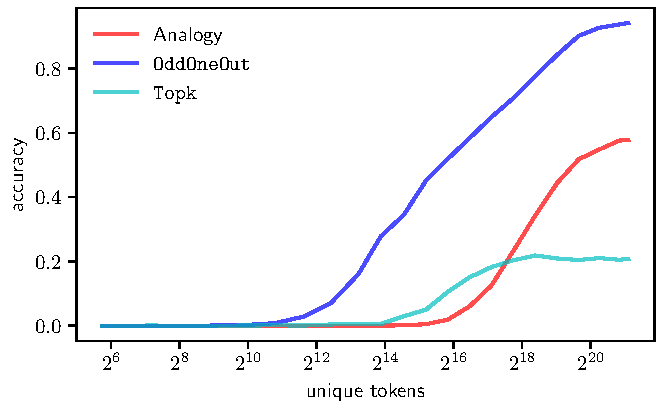
\includegraphics[width=1\columnwidth]{size_vs_acc.pdf} 
\caption{
    %The plot above compares the regions of effectiveness for our evaluation metrics. 
    The standard analogy task \citep{mikolov2013efficient} fails to measure the quality of word embeddings trained on small datasets,
but our novel $\OddOneOut$ and $\topk$ tasks succeed in this regime.
%Though $\OddOneOut$ seems the clear victor of these methods, experimentation in \ref{sec:mca} shows that $\topk$ works better in some circumstances.
%Full experimental details are given in Section \ref{sec:experiments:eng}.
}
\label{fig:size_vs_acc}
\end{figure}

With this analogy test set in hand,
you train dozens of models with varying hyperparameters.
Unfortunately, all these models get 0 accuracy on your test set.
You simply don't have enough data to get good results on the analogy task.
As Figure \ref{fig:size_vs_acc} shows,
the analogy task requires a large training dataset before it begins getting non-zero results.
(Further details are provided in Section \ref{sec:experiments:eng} below.)
But that does not mean that you cannot train word embeddings on Middle English.

In this paper,
we introduce the $\OddOneOut$ and $\topk$ tasks for evaluating word vectors on low-resource languages, 
and successfully train word embeddings for Middle English, 15 other extinct languages, and a low-resource emoji embedding task.
To get a sense of scale, the original word2vec paper trained English word embeddings on a dataset with 6 billion tokens \citep{mikolov2013efficient} and subsequent work has improved performance by training on datasets as large as 630 billion tokens \citep{grave2018learning}. 
In this paper, the largest dataset we consider has 41 million tokens,
and the smallest only 1813 tokens.
We argue that different evaluation techniques are needed for datasets like ours that are more than 1000 times smaller,
and Figure \ref{fig:size_vs_acc} shows that the $\OddOneOut$ and $\topk$ tasks can measure improvement in word embedding quality with much smaller datasets than the analogy task.

Other work in the low-resource regime has focused on developing new training methods rather than evaluation methods.
Specifically, the goal is to reduce the sample complexity of word embedding models by adding new regularizations \cite{adams-etal-2017-cross,jiang2018learningword,gupta-etal-2019-improving,jungmaier-etal-2020-dirichlet}.
A common thread of this work is the difficulty of evaluation.
Unfortunately, each of these works evaluate their method only in a simulated low-resource environment using modern English text and not on any actual low-resource languages.
They do this specifically because no evaluation metrics were available that were suitable for their low-resource target languages.
More theoretical work has also shown that these simulated low-resource design methodologies give biased hyperparameter estimates which systematically overestimate model performance \citep{kann-etal-2019-towards}.
This highlights the need for new evaluation methods like ours suitable for the low-resource regime.

High-resource languages also directly benefit from our methods in two ways.
First, we help automate evaluation on many languages.
\citet{grave2018learning} trained FastText embeddings on 157 languages using data from the Common Crawl project.
But they were only able to explicitly evaluate 10 of these language models using the analogy task due to the expense required in developing appropriate test sets.
We introduce a method that automatically generates test sets for our $\OddOneOut$ and $\topk$ methods in any of Wikidata's 581 supported languages (which includes extinct languages like Middle English).%
%\footnote{For the full list of languages supported, see \url{https://www.wikidata.org/wiki/Help:Wikimedia_language_codes/lists/all}}

Second, many applications of word embeddings investigate low-resource subsets of high-resource languages.
There is growing body of digital humanities work where English language text is subdivided into smaller corpora based on time periods \cite[e.g.][]{kulkarni2015statistically,hamilton2016diachronic,hamilton2016cultural,dubossarsky2017outta,szymanski2017temporal,chen2017understanding,liang2018dynamic,tang2018state,kutuzov2018diachronic,kozlowski2019geometry}
or different political ideologies \citet{azarbonyad2017words}.
Word embeddings are then trained on these smaller corpora,
and differences in the resulting embeddings are used to track how word usage changes.
Our evaluation methods can be used to improve the ability to evaluate this work as well.

Our contributions can be summarized with the following three points.

\label{sec:contributions}
\begin{enumerate}
    %\item 
    %We show that the analogy task introduced by \citet{mikolov2013efficient} is not suitable for evaluating low-resource word embeddings.
    \item 
    We introduce the first word embedding evaluation tasks designed specifically for the low-resource setting, $\OddOneOut$ and $\topk$.
    Code for computing these metrics is released as an open source Python library.%
    \footnote{
        URL hidden for blind review.
    }
    \item 
    We introduce a method for automatically generating test datasets for the $\OddOneOut$ and $\topk$ tasks in the 581 languages supported by the wikidata project.
        %\footnote{For the full list of languages supported, see \url{https://www.wikidata.org/wiki/Help:Wikimedia_language_codes/lists/all}}
    All previous evaluation methods work on only a small number of languages (typically just English),
    and require significant manual work to adapt to new languages.
	\item 
    We perform the largest existing multilingual evaluation on low-resource languages using 16 extinct languages from the Classical Languages ToolKit (CLTK) library \citep{johnson2014}.
    We evaluate these word embeddings on a qualitative downstream task that investigates how religious words are used in each language.
    %Specifically, we provide word embeddings for the 16 of the 18 languages in the Classical Languages ToolKit (CLTK) library \citep{johnson2014}.
    %We further introduce a new downstream task called the Language Comparison Task (LCT) that lets us map which topics are included in these classical language corpora.
\end{enumerate}

The remainder of the paper is organized as follows.
Section \ref{sec:method} formally defines the $\topk$ and $\OddOneOut$ tasks.
Section \ref{sec:experiments} empirically demonstrates that these tasks are better than the analogy task in low-resource settings.
We use a synthetic English language experimental design common in previous work,
and demonstrate the versatility of our evaluation metrics by applying them to an emoji embedding task for which the analogy task is not even well defined.
Section \ref{sec:mca} computes word embeddings for 16 extinct languages.
We further introduce our technique for using wikidata to automatically generate the test sets for the $\OddOneOut$ and $\topk$ tasks and the LCT task and provide a semantic analysis of the topics covered in each of the 16 language corpora.
Section \ref{sec:discussion} concludes by discussing how extensions to this work could serve communities working with low-resource languages.

\fixme{Figure 1: Change the x-axis to ``training dataset size (number of unique tokens)''; also, the font is a bit small}

\section{Evaluation Methods}
\label{sec:method}
The $\OddOneOut$ and $\topk$ tasks are simple and widely applicable.
Both tasks require a test set consisting of a list of categories,
where each category contains a list of words that belong to that category.
Table \ref{table:wikidata} shows some example categories generated through a fully automated process (described in Section \ref{sec:wikidata}).
%For example, the category \texttt{ancient\_cities} might contain the words \texttt{carthage}, \texttt{sparta}, and \texttt{persepolis}.
%\fixme{add greek translations?}
The $\topk$ task measures a model's ability to identify words that are related to each category,
and conversely the $\OddOneOut$ task measures a model's ability to identify words that are unrelated to each category,

Formally,
assume that there are $m$ categories,
that each category has $n$ words%
\footnote{
    In practice, the number of words per category can vary for each category,
    however for notational simplicity we assume that each category has the same number of words.
},
that there are $v$ total words in the vocabulary,
and that the words are embedded into $\mathbb {R}^d$.
The method of generating the embedding (e.g.\ word2vec, GloVe, FastText) does not matter.
Let $c_{i,j}$ be the $j$th word in category $i$,
and let $C_i = \{c_{i,1}, c_{i,2}, ..., c_{i,n}\}$ be the $i$th category.

\subsection{The $\topk$ method}
Let $\FindMostSimilar(k,w)$ return the $k$ most similar words in the vocabulary to $w$.
We use the cosine distance in all our experiments,
but any distance metric can be used.
Next, define the $\topk$ score for class $i$ to be
\begin{equation}
    \topk(k,i) = \frac{1}{n}\sum_{j=1}^n \frac{1}{k}\sum_{\mathrlap{x \in \FindMostSimilar(k, c_{i,j})}} \indicator{x \in C_i}
\end{equation}
and the $\topk$ score for the entire evaluation set to be
\begin{equation}
    \topk(k) = \frac{1}{m}\sum_{i=1}^m \topk(k,i)
    .
\end{equation}

The runtime of $\FindMostSimilar$ is $O(dvk)$.\footnote{
    We use GenSim's implementation of $\FindMostSimilar$,
    which uses the naive loop strategy for computing the nearest neighbor.
    Data structures like the $k$d-tree or cover tree could potentially be used to speed up this search,
    but we did not find such data structures necessary.
}
So the runtime of $\topk(k,i)$ is $O(dnk^2v)$
and the runtime of $\topk(k)$ is $O(dnmk^2v)$.
Typically $k$ is small (we recommend $k=3$ in our experiments),
and so the runtime is linear in all of the interesting parameters.
In particular, it is linear in both the size of our vocabulary, the number of categories in the test set, and the size of the categories.

\subsection{The $\OddOneOut$ method}
Define the $\OddOneOut$ score of a set $S$ with $k$ words with respect to a word $w\not\in S$ as

%\begin{equation}
%    \OddOneOut(S,w) = \indicator{w = \hat w},
%\end{equation}
%where
%\begin{equation}
%    \hat w = \argmax_{x \in S\cup\{w\}} \ltwo{x - \mu}
%    \quad
%    \text{and}
%    \quad
%    \mu = \frac1{k+1}\bigg(w + \sum_{i=1}^k{s_i}\bigg)
%    .
%\end{equation}

\begin{equation}
    \OddOneOut(S,w) = \indicator{w = \hat w},
\end{equation}
where
\begin{equation}
    \hat w = \argmax_{x \in S\cup\{w\}} \ltwo{x - \mu}
\end{equation}
\begin{equation}
    %\quad
    \text{and}
    \quad
    \mu = \frac1{k+1}\bigg(w + \sum_{i=1}^k{s_i}\bigg)
    .
\end{equation}


We define the $k$th order $\OddOneOut$ score of a category $i$ to be
\begin{equation}
    \OddOneOut(k,i) = \frac 1 {|P|} \sum_{\mathclap{(S,w) \in P}} \OddOneOut(S,w)
    \label{eq:OOOki}
\end{equation}
where
\begin{multline}
    P = \{ (S, w) : S \text{~is a combination of $k$ words}\\\text{from $C_i$}, \text{and~} w \in V-C_i \}
    .
    \label{eq:P}
\end{multline}
In Equation \eqref{eq:P} above,
the total number of values that $S$ can take is ${n \choose k} = O(n^k)$,
and the total number of values that $w$ can take is $O(v)$,
so $|P| = O(n^kv)$.
Finally, we define the $k$-th order $\OddOneOut$ score of the entire evaluation set to be
\begin{equation}
    \OddOneOut(k) = \frac 1 m \sum_{i=1}^m \OddOneOut(k,i)
    .
\end{equation}

The runtime of $\OddOneOut(S,w)$ is $O(dk)$.
So the runtime of $\OddOneOut(k,i)$ is $O(dkn^kv)$ and the runtime of $\OddOneOut(k)$ is $O(dkmn^kv)$.
This exponential dependence on $k$ is very bad.
In practice, we used $k=3$ in all of our experiments,
but even this small value required prohibitively long run times.

%Comparing the runtimes of $\OddOneOut(k)$ and $\topk(k)$, we can see that $\OddOneOut(k)$ is a factor of $O(m^{k-1}k^{-1})$ slower.
%In real world applications, $m >\!\!> k$, and so $\OddOneOut$ will take considerably more time to compute.
%In particular, the Mikolov test evaluations in Section \ref{sec:experiments} below use $m=50$ and $k=3$,
%so the $\OddOneOut(k)$ score takes approximately 800x longer to compute.

To solve this problem, we use a sampling strategy.
Let $\tilde P$ denote the set of $p$ samples without replacement from the set $P$.
Then we rewrite Equation \ref{eq:OOOki} as
\begin{equation}
    \OddOneOut(k,i) = \frac 1 p \sum_{\mathclap{(S,w) \in \tilde P}} \OddOneOut(S,w)
\end{equation}
With this definition, the runtime of $\OddOneOut(k)$ is $O(dkmpv)$,
which is linear in all the parameters of interest.
In our experiments, we found $p=1000$ to give sufficiently accurate results without taking too much computation.

\section{Experiments}
\label{sec:experiments}

We demonstrate the usefulness of our evaluation metrics with two experiments.
First, we show that the $\OddOneOut$ and $\topk$ metrics are better measures of word embedding quality than the $\analogy$ metric in the low-resource regime using simulated English data.
Second, we show that the $\OddOneOut$ and $\topk$ metrics are useful for model selection in an emoji embedding task where the analogy task is not well defined.
This experiment also demonstrates that the $\OddOneOut$ and $\topk$ metrics correlate with downstream task performance.

\subsection{English Experiments}
\label{sec:experiments:eng}

This experiment measures the performance of the $\OddOneOut$, $\topk$, and $\analogy$ metrics as a function of data set size.

%Figure \ref{fig:data_vs_methods} shows the results of the evaluation of these models on three intrinsic tasks-- \texttt{Analogy}, \texttt{OddOneOut}, and \texttt{Topk}.
 %We see that for the various tasks both \texttt{OddOneOut} and \texttt{Topk} start to see an increase in performance with roughly $32x$ less data compared to \texttt{Analogy}. 
 %In addition, though the shapes are roughly similar, the curve for \texttt{OddOneOut} and \texttt{Topk} have steeper slopes before plateauing, 
 %indicating a greater sensitivity to amount of data.
  %Overall, these findings suggest that in the low resource scenarios, the analogy task does will not always provide adequate intrinsic evaluation for word embeddings,
  %especially compared to these simpler methods.

For training data, we use a 2017 dump of the English-language Wikipedia 
that contains 2 billion total tokens and 2 million unique tokens.
The dataset is freely distributed with the popular GenSim library \cite{rehurek_lrec} for training word embeddings,
and it is therefore widely used.
State-of-the-art embeddings are trained on significantly larger datasets---%
for example, datasets based on the common crawl contain hundreds of billions of tokens even for non-English languages \cite{buck2014n,grave2018learning}---%
but since our emphasis is on the low-resource setting,
this 2 billion token dataset is sufficient.

Using the wikipedia dataset, we generate a series of synthetic low-resource datasets of varying size.
First, we sort the articles in the wikipedia dataset randomly.%
\footnote{
    This sorting is required for our low-resource datasets to be representative of English language text.
    Without this random sorting step,
    most of our datasets would be based only on articles that begin with the letter \texttt{A},
    and therefore would not contain a representative sample of English words.
 %This is a problem because larger models would have the benefit of both greater amounts of data as well as a greater contextual variety of data compared to smaller ones. 
 %To mitigate this bias we use a linear congruential generator to randomly stream the training data in a way that is reproducible. 
 %Thus, in addition to mitigating model bias tied to the content of training data, our random generator also ensures that each model uses a subset of the training data of models larger than it.
}
Then, each dataset $i$ contains the first $2^i$ tokens in the randomly ordered wikipedia dump.

On each of these low-resource datasets,
we train a word2vec skipgram model with GenSim's default hyperparameters\footnote{
Embedding dimension 100, number of epochs 1, learning rate 0.025, window size is 5, min count is 5.
},
which are known to work well in many contexts.
Importantly, we do not tune these hyperparameters for each low-resource dataset.
Instead, we use the same hyperparameters because our goal is to isolate the effects of dataset size on the three evaluation metrics.

\begin{figure}
\centering
%    \resizebox{6in}{3in}{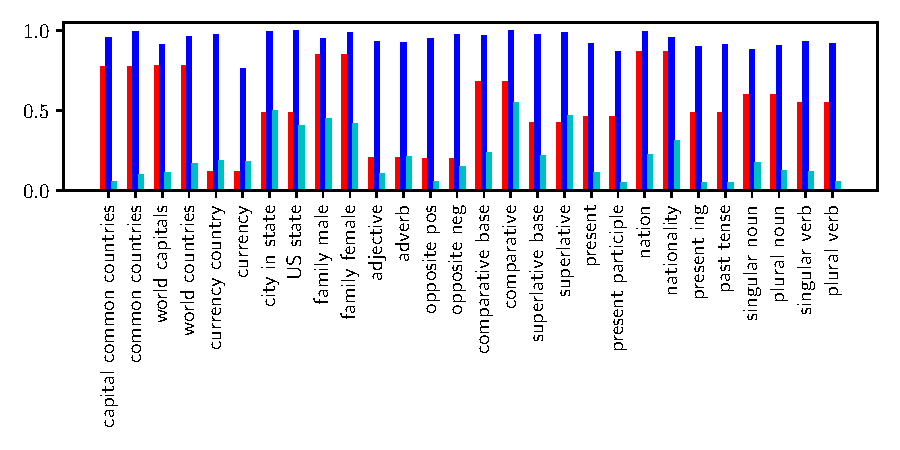
\includegraphics{cross_cat_acc.pdf} }
    \resizebox{!}{4.95in}{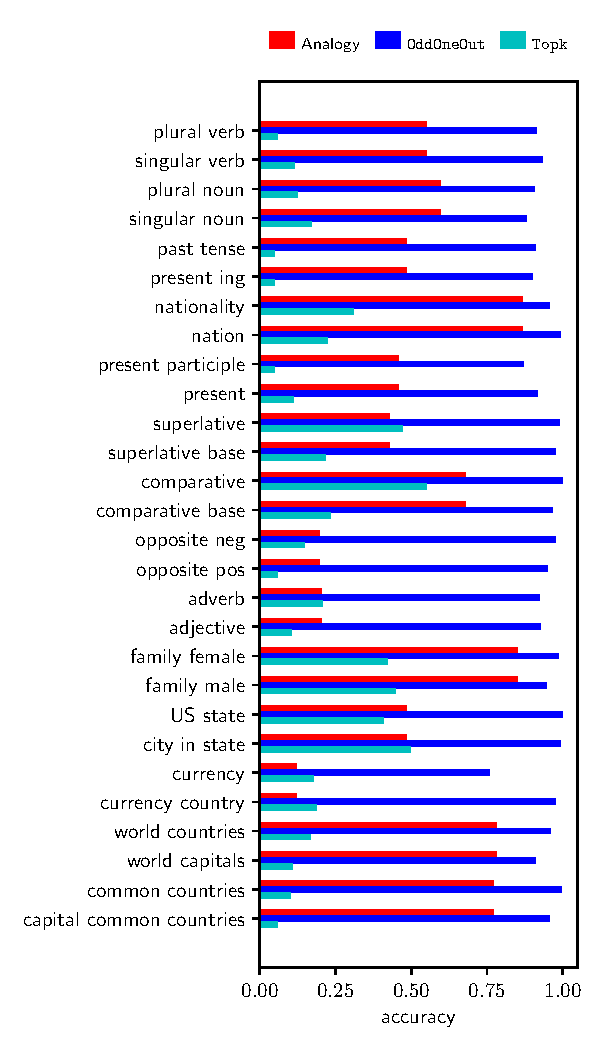
\includegraphics{cross_cat_acc-horizontal.pdf} }

\caption{
    Breakdown of model performance by category.
    There does not appear to be any correlation between the performance of the three tasks,
    indicating that each task is measuring a different aspect of linguistic knowledge.
    \fixme{the category column should be labeled as ``categories'' and the key should be labeled as ``tasks''}
    %The methods perform better on some categories than others. $\topk$  seems to excel in categories that are more homogenous like 'family female',
 %while analogies seem to work best with geographical relationships.
  %Note that in adapting the Google analogy set to work with our methods required splitting each relationship pair into two separate categories. 
  %As a result the analogy score for a given relationship is shown twice;
   %one bar in each of the categories that make up the pair.
   }
\label{fig:cross_cat_acc}
\end{figure}

For the analogy task, we use the standard Google Analogy Test Set introduced by \citep{mikolov2013efficient}.
This test set contains 14 sets of analogies,
and each analogy set contains 2 categories that are being compared.
We generate test sets for the $\OddOneOut$ and $\topk$ tasks from all 28 categories in the Google test set.
For example,
the countries-capitals analogy set has analogies like
%\begin{equation}
%\texttt{England} - \texttt{London} + \texttt{Paris} \approx \texttt{France}
%\end{equation}
\begin{quote}
    ~\!\!\!\!\!\!\emph{London is to England as Paris is to France}
\end{quote}
comparing countries and capitals.
We use the set of all countries as one category and the set of all capitals as a separate category in the $\OddOneOut$ and $\topk$ test sets.
Note that in this dataset conversion, we are explicitly losing information about how these categories relate to each other.
Note that the analogy task tests a model's knowledge about each category and how these categories relate to each other,
whereas the $\OddOneOut$ and $\topk$ tasks will only test a model's knowledge about each category individually.
Since these tasks are testing less knowledge,
it makes since that they will get improved performance on smaller data sets.
This intuition is confirmed in the results shown in Figure \ref{fig:size_vs_acc}.
Figure \ref{fig:cross_cat_acc} shows a breakdown in accuracy by category on the model trained on the full dataset.
How a category performs on one task does not seem correlated to how a model performs on other tasks,
which indicates that all three tasks are in fact measuring different aspects of linguistic knowledge (and not just representing the same knowledge scaled differently).

\subsection{Emoji Experiments}
\begin{figure}
\centering
    \resizebox{\columnwidth}{!}{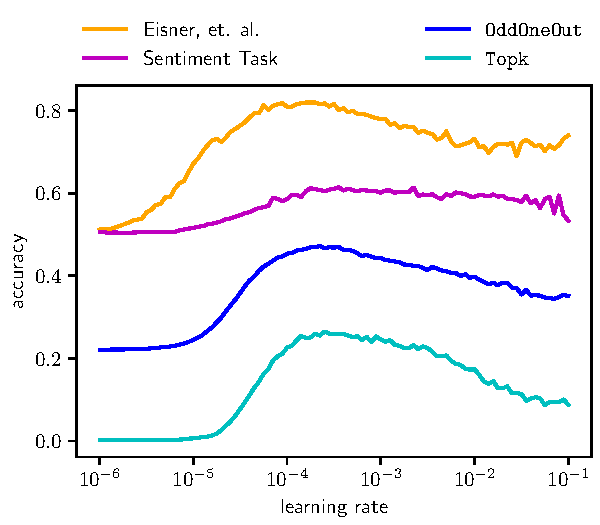
\includegraphics{emoji_exp.pdf} }
\caption{
    The performance of the generic $\OddOneOut$ and $\topk$ tasks mirrors the performance of \citet{eisner2016emoji2vec}'s emoji-specific model selection task as the learning rate varies.
    All three tasks provide can be used to estimate the optimal learning rate for the downstream sentiment classification task.
}
\label{fig:emoji}
\end{figure}

This second experiment demonstrates the versatility of our methods by applying them to the domain of emoji embeddings.
We show that our generic $\topk$ and $\OddOneOut$ metrics perform as well as a custom designed emoji evaluation metric.
That is, we don't sacrifice performance by choosing our easy-to-use and widely applicable metrics over harder-to-use domain-specific metrics.

Emoji embeddings are an important topic of study because they are used to improve the performance of sentiment analysis systems \cite[e.g.][]{eisner2016emoji2vec,felbo2017using,barbieri2017emojis,ai2017untangling,wijeratne2017semantics,al2019smile}. 
Unfortunately,
the standard analogy task is not suitable for evaluating the quality of emoji embeddings for two reasons.
First, emoji embeddings are inherently low-resource---%
only 3000 unique emojis exist in the Unicode standard---%
and thus evaluation techniques specifically designed for the low-resource setting will be more effective.
Second, the semantics of most emojis do not allow them to be used in any analogy task.
In particular, the original emoji2vec paper \cite{eisner2016emoji2vec} identifies only 6 semantically meaningful emoji analogies.

In order to tune their emoji embeddings, \citet{eisner2016emoji2vec} therefore do not use the analogy task,
and instead introduce an ad-hoc ``emoji-description classification'' metric that required the creation of a test set with manually labeled emotion-description pairs.
Due to the expense of manually creating this test set,
only 1661 of the 3000 Unicode emojis are included.%
\footnote{New emojis have been added to the Unicode standard since the publication of \citet{eisner2016emoji2vec},
but these emojis have not been added to the test set.
}
The $\topk$ and $\OddOneOut$ metrics improve on the ``emoji-description classification'' metric because they are able to evaluate the quality of all emojis and require no manual test set creation.
For our test set categories, we use the categories that the Unicode standard provides for each emoji.%
\footnote{For the full list of categories, see \url{https://unicode.org/Public/emoji/13.0/emoji-test.txt}}

To test the performance of the three metrics,
we use them to tune the hyperparameters of an emoji2vec model.
To ensure the fairest comparison possible, we use the original emoji2vec code for training and model selection,
changing only the function call to the metric used.
In particular, this means we are only embedding and evaluating on the subset of 1661 emojis supported by the ``emoji-description classification'' metric.
The code allows tuning the model's learning rate, \fixme{insert other options here}.
We found that the learning rate was the only hyperparameter to have a significant impact,
and Figure \ref{fig:emoji} shows how the learning rate effects the performance on the three evaluation metrics and the performance on a downstream sentiment analysis task.
All three metrics show optimal performance with a learning rate of approximately $8\times10^{-4}$,
which also results in the best performance on the downstream task.
This indicates that our $\topk$ and $\OddOneOut$ metrics generate the same models as the specialized ``emoji-description classification'' metric,
but our metrics have the advantage of being simpler, more widely applicable, and easier to generate test data for.

Note that it is incorrect to conclude that the \citet{eisner2016emoji2vec} method is better than the $\OddOneOut$ and $\topk$ values because it achieves higher accuracy rates in Figure \ref{fig:emoji}.
When evaluating a model selection metric,
the important point to consider is the location where the metric is maximized,
and not the maximum value itself.
The location is used to determine the optimal hyperparamter,
and all three metrics have maximal performance at the same location.

\section{Multilingual Content Analysis}
\label{sec:mca}

In this section we perform the first highly multilingual analysis of word embeddings for low-resource languages.
We analyze 18 languages provided by the Classical Languages ToolKit (CLTK) library \citep{johnson2014}.%
\footnote{
    Specifically, we analyzed all languages for which CLTK provides both a training corpus and a tokenization function,
    as these are the minimum requirements needed for training word embeddings.
}
Each of these languages is ``extinct'' in the sense that no new native text will ever be generated in these languages.
To get better models on these languages, it is impossible to collect more data,
we must develop better techniques for the low-resource setting.
The largest of these language datasets is Ancient Greek, with 37.8 million tokens,
and the smallest is Ancient Gujarati with only 1813 tokens.
Our techniques successfully let us choose hyperparameters for 16 of the 18 languages under consideration,
including for the tiny Ancient Gujarati model.

First we describe a procedure for automatically generating test set data for the $\OddOneOut$ and $\topk$ tasks using wikidata.
Then, we describe our model training and selection procedure for each language.
Finally, we perform the LCT task and perform an interlanguage analysis of the corpora's content.

\begin{figure}
%\centering
%\begin{tabular}{lllllllll}
%\toprule
%\multicolumn{3}{l}{Biblical Figures} & \multicolumn{3}{l}{Facets of Buddhism} & \multicolumn{3}{l}{Facets of Hinduism} \\
 %%Abraham & אברהם & ઇબ્રાહિમ & Buddha  & בודהה & બુદ્ધત્વ & Mahātmā & - & મહાત્મા \\
 %%Hilkiah &  חלקיה & - & Vipassanā & ויפאסנה & વિપ્શના & Rishi & - & ઋષિ\\
 %%Matthew the Apostle & מתי & - & Bhagavan & - & ભગવાન & Hindu prayer beads & - & જપમાળા \\
 %%Zerubbabel & זרובבל בן שאלתיאל  & - & meditation & מדיטציה & - & Ashvamedha & - & અશ્વમેધ યજ્ઞ\\
 %%Joseph & יוסף הקדוש  & જોસેફ & nirvana & נירוואנה &  નિર્વાણ & Brahmin & - & બ્રાહ્મણ\\
%\end{tabular}
%\includegraphics[width=\textwidth,height=2in]{example-image-a}

\small
\itshape
%\centering
    \begin{tabular}{p{0.9\columnwidth}}
    \textbf{Biblical Figures:}
    Abraham,
    Hilkiah,
    Matthew the Apostle,
    Zerubbabel,
    Joseph
    \\
    \\[-4pt]

    \textbf{Facets of Buddhism:}
    Buddha,
    Vipassan,
    Bhagavan,
    meditation,
    nirvana
    \\
    \\[-4pt]

    \textbf{Facets of Hinduism:}
    Matm,
    Rishi,
    Hindu prayer beads,
    Ashvadamedha,
    Brahmin
    \\
    \\[-4pt]
\end{tabular}

\caption{
    Example categories and terms for our test set that we automatically extracted from Wikidata.
    Only the English translations are shown.
    \fixme{include 10-15 (exactly 3 lines each) alphabetically ordered}
    \fixme{are these the exact names in wikidata?  I couldn't find the categories in google}
}
\label{table:wikidata}
\end{figure}


\begin{table*}[t]
\centering
    %\resizebox{\textwidth}{!}{
\scriptsize
\begin{tabular}{lrrllrrrrlrrr}
\toprule
    \multicolumn{3}{c}{\bf Corpus} & \multicolumn{7}{c}{\bf Hyperparameters $^{(*)}$} & \multicolumn{3}{c}{\bf Metrics} \\
\cmidrule(lr){1-3}\cmidrule(lr){4-10}\cmidrule(lr){11-13}
%\midrule
 \multicolumn{1}{l}{Language} & \multicolumn{1}{r}{Total Tokens} & \multicolumn{1}{r}{Uniq. Tok.} & \multicolumn{1}{l}{Model} & \multicolumn{1}{l}{Type} & \multicolumn{1}{r}{Dim} & \multicolumn{1}{r}{WS} & \multicolumn{1}{r}{LR} & \multicolumn{1}{r}{MC} & \multicolumn{1}{c}{Lem} & \multicolumn{1}{c}{\tiny$\OddOneOut$} & \multicolumn{1}{c}{$\topk$} & \multicolumn{1}{c}{\texttt{ Avg}} \\
    \midrule
    Helenic&&&&&&&&&&&&\\
%\midrule
 \quad Anc. Greek & \num{37868209} & \num{1877574} & w2v & cbow &  \num{40} &  \num{9} &  \num{.1} &  \num{4} & False & \num{0.1900} & \num{0.0178} & \num{0.0327}\\
%    & greek & modern greek & \num{37868209} & \num{1877574} & fast & sg & 90 & 7 & -1 & 5 & True & 300 & 9 & 19.36\\  
%    \midrule
    &&&&&&&&&&&&\\[-4pt]
    Italic&&&&&&&&&&&&\\
%    \midrule
 \quad Latin & \num{17777429} & \num{470790} & w2v & cbow &  \num{50} &  \num{10} &  \num{.1} &  \num{7} & False &  \num{0.1527} &  \num{0.0645} &  \num{0.0908}\\ 
   \quad Old French  & \num{68741} & \num{8343} &  fast & sg & \num{250} & \num{6} & \num{.1} & \num{8}  & False & \num{0.0001} & \num{0.0109} & \num{0.0003}\\
%    \midrule
    &&&&&&&&&&&&\\[-4pt]
%\multicolumn{13}{l}{Germanic}\\
    Germanic &&&&&&&&&&&& \\
%    \midrule
\quad Mid. English & \num{7048144} & \num{314527} & fast & sg & \num{90} & \num{5} & \num{.1} & \num{7} & False & \num{0.0239} & \num{0.0012} & \num{0.0024} \\
   \quad Mid. High German & \num{2090954} & \num{60674} & fast & cbow & \num{15} & \num{6} & \num{.1} & \num{3} & False & \num{0.0005} & \num{0.0029} & \num{0.0010} \\
   \quad Old English  & \num{104011} & \num{33018} & fast & cbow & \num{425} & \num{3} & \num{.1} & \num{3} & True & \num{0.0000} & \num{0.0005}  & \num{0.0002} \\
   \quad Old Norse & \num{458377} & \num{59186} & w2v & cbow & \num{60} & \num{10} & \num{.1} & \num{3} & False & \num{0.0569} & \num{0.0093} & \num{0.0161} \\
   \quad Old Swedish & \num{1297740} & \num{116374} &  fast & sg & \num{50} & \num{8} & \num{.1} & \num{5} & False & \num{0.0031} & \num{0.0001} & \num{0.0004} \\
%    \midrule
    %\multicolumn{13}{l}{}\\[-4pt]
    %\multicolumn{13}{l}{Indic}\\
    &&&&&&&&&&&&\\[-4pt]
    Indic&&&&&&&&&&&&\\
%    \midrule
\quad Bengali & \num{5539} & \num{2323} & fast & cbow & \num{15} & \num{3} & \num{.1} & \num{4} & False & \num{0.0000} & \num{0.0065} & \num{0.0002} \\
   \quad Gujarati & \num{1813} & \num{1140} & fast & sg & \num{80} & \num{3} & \num{.1} & \num{5} & False & \num{0.0000} & \num{0.0292} & \num{0.0002} \\
   \quad Hindi & \num{587655} & \num{55483} & fast & cbow & \num{45} & \num{4} & \num{.1} & \num{8} & False & \num{0.0175} & \num{0.0038} & \num{0.0064}\\
   \quad Malayalam & \num{9235} & \num{5405} & - & - & - & - & - & - & - & - & - & - \\
    \quad Marathi  & \num{797926} & \num{96778} & w2v & sg & \num{400} & \num{4} & \num{.1} & \num{6} & False & \num{0.0214} & \num{0.0065} & \num{0.0101} \\
    \quad Punjabi & \num{1024075} & \num{31343} & fast & sg & \num{50} & \num{8} & \num{.1} & \num{5} & False & \num{0.0000} & \num{0.0001} & \num{0.0001} \\
    \quad Sanskrit & \num{4042204} & \num{896480} & w2v & sg & \num{35} & \num{9} & \num{.1} & \num{10} & False & \num{0.1391} & \num{0.0093} & \num{0.0175}\\
    \quad Telugu & \num{537673} & \num{276330} &  w2v & cbow & \num{60} & \num{10} & \num{.1} & \num{3} & False & \num{0.0042} & \num{0.0000} & \num{0.0002} \\
%    \midrule
    %\multicolumn{13}{l}{}\\[-4pt]
    %\multicolumn{13}{l}{Semitic}\\    
    &&&&&&&&&&&&\\[-4pt]
    Semitic&&&&&&&&&&&&\\
%    \midrule
  \quad Classical Arabic & \num{81306} & \num{20493} & - & - & - & - & - & - & - & - & - & - \\
   \quad Hebrew & \num{41378460} & \num{893512} & fast & sg & \num{30} & \num{4} & \num{.1} & \num{3} & False & \num{0.0646} & \num{0.0056} & \num{0.0104} \\ 
\bottomrule
\end{tabular}
%}

    \vspace{0.1in}
    $(*)$ w2v = word2vec, fast = fastText, sg = skipgram, Dim = Dimension, WS = Window Size, LR = Learning Rate, MC = Min Count, Lem = Lemmatization

\caption{
    The optimal hyperparameters selected for training a model on each corpus,
    and their corresponding evaluation metrics.
    ($\texttt{Ave}$ denotes the hyperbolic mean of $\OddOneOut$ and $\topk$.)
    We successfully trained models on 16 of the 18 languages provided by the CLTK library (everything except Malayalam and Classical Arabic).
    Previously, word embeddings had only been trained on Ancient Greek and Latin.
    %The table above provides details for the best model trained for languages supported by CLTK.
%Following a tuning process, models were chosen by their $\texttt{Combined Score}$
%which is calculated as the harmonic mean of $\topk$ and $\OddOneOut$.
%It is important to note that the absolute score for our evaluation metrics are not important in and of themselves,
%rather they are important as indicators of a change in embedding quality that the analogy task would fail to show.
%To emphasize this, we have reported the raw number of correct answers for each metric.
%Using $\OddOneOut$ and $\topk$ allows us to tune models trained on corpora with unique token counts in the thousands instead of the millions.
    }
\label{table:language}
\end{table*}

\subsection{Test Set Generation with Wikidata}
\label{sec:wikidata}

One of the most difficult and time consuming steps of evaluating word embeddings on a new language is generating a high quality test set for this language.
We now present the first fully automatic way to generate these test sets.
Our method uses Wikidata\footnote{\url{https://wikidata.org}},
which is the knowledge base that powers Wikipedia
and contains millions of items and their semantic relationships.
Wikidata supports 581 languages,
and our test set generation method works for all of them.
This method does not work for generating analogy test sets,
but only works for generating the category test sets needed for our $\OddOneOut$ and $\topk$ tasks.
We implement this process using the Wikidata Query Service and SPARQL in our open source Python library,
making it easy to generate arbitrary test sets.

The idea is straightforward.
Some items in Wikidata actually represent categories,
and other items can be an ``instance of'' these categories.
For example, item \texttt{Q20643955} (the category of ``Human Biblical Figures''),
and item \texttt{Q9181} (the Biblical patriarch ``Abraham'') is an instance of \texttt{Q20643955}.
We can then generate a category of ``Human Biblical Figures'' by gathering all the items that are an instance of this category,
and extracting the translation of these items into our chosen language.

There are two minor complications to the process above.
First, the item may not have a translation into all languages.
Item \texttt{Q3276278} (the minor Hebrew prophet Hilkiah), for example, does not have a translation into any of the languages we are studying except for Hebrew.
We replace all of these words with a special out-of-vocabulary token.
During the evaluation tasks,
the models will be guaranteed to miss any test case involving these words.
This will cause the model's performance to decrease,
but it will not cause the optimal set of hyperparameters to change because the model's performance will decrease uniformly for all hyperparameters.
This is acceptable because our primary goal with the $\OddOneOut$ and $\topk$ metrics is model selection.

Second, the item may have a multi-word translation.
Item \texttt{Q43600} is translated into English as ``Mathew the Apostle'' which is guaranteed to be out of vocabulary because our embeddings are only for individual words and not phrases.
We handle this case simply by treating phrases the same way we would treat any other out of vocabulary word for these models.
For a word2vec model, these phrases are commonly replaced by a single out of vocabulary token,
but FastText models incorporate sub-word information are therefore able to generate reasonable vectors that are good representations of these phrases.
We therefore expect FastText models to perform better on datasets with many multi-word translations.

In this paper we focus on three wikidata categories that we hypothesized would be relevant to the languages in CLTK we are studying:
\texttt{Q20643955} (Biblical Figures),
\fixme{\texttt{???}} (Facets of Hinduism),
and \fixme{\texttt{???}} (Facets of Buddhism).
Table \ref{table:wikidata} shows representative examples from each category.
The categories are large, with between 100-400 items each, and so we do not reproduce the full categories here.

%Using Wikidata we were able to reconstruct all of the semantic categories contained within the Google analogy set with the option of greater customization and more categories.
%Additionally, Wikidata supports the translation of queried items into 461 languages, allowing test sets to easily be converted between languages.
%Though not all items have translated labels in all 461 languages, support is quite extensive and will only get better. 
%\fixme{Is 461 correct?}
%
%One of the disadvantages of using Wikidata is that syntactic categories are much harder to construct;
%however, since semantic categories are usually more difficult to generate 
%and require more arbitrary decisions this approach is still very valuable.
%
%\fixme{What are the exact categories used?}
%
%\fixme{Does the library allow the easy construction of these categories?}

\subsection{Model Selection}

\begin{figure*}
\centering

\resizebox{\textwidth}{1.5in}{
\begin{tabular}{lccc}
\multicolumn{3}{l}{Language} &\multicolumn{1}{c}{\hspace{4em} Category} \\ 
\multicolumn{4}{l}{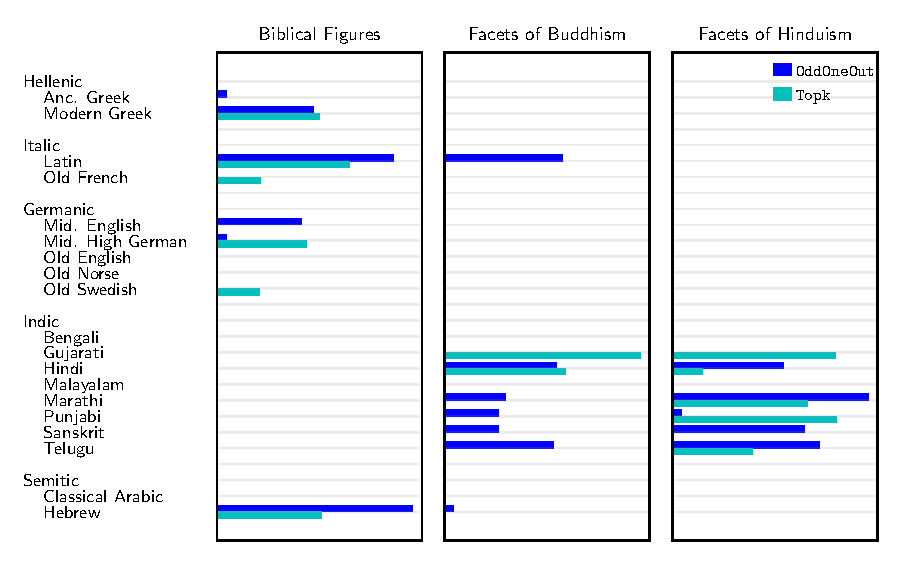
\includegraphics{lct-biblical.pdf}} \\
\end{tabular}
}

\caption{
    \fixme{}
    %(\textbf{Top})
    %High performance on the Biblical Figures category indicates some level of biblical influence via the corpus. 
    %Interestingly, we see that greek embeddings optimized on the Modern Greek test set significantly outperformed the embeddings optimized for the Ancient Greek. 
    %This matches our intuition that things of a biblical nature have had a greater influence on Modern Greek than Ancient Greek.
    %(\textbf{Middle})
    %Though many of the Indic language embeddings performed well on the Facets of Buddhism, 
    %surprisingly so did our Latin and Hebrew embeddings. 
    %This leads us to believe that some Buddhist concepts and words are shared by corpora spanning languages as diverse as Hebrew, Latin, and Hindi. 
    %At the same time, it should also be noted that Latin and Hebrew were two of the largest models trained compared to other classical languages and thus also likely benefit from greater resource richness.
    %(\textbf{Bottom})
    %Similar to Figure \ref{fig:biblical} we see languages more closely related to the topic of the category achieving better performance, in this case primarily the Indic languages. 
    %Interestingly, our Bengali embeddings performed poorly on this category suggesting that the corpus did not refer heavily to the Hindu context.
}
\label{fig:downstream}
\end{figure*}

%% Improved Table - raw scores
%\begin{table*}[t]
%\centering
%%\scalebox{.54}{
%\scriptsize
%\begin{tabular}{lrr|llrrrrl|rrr}
%\toprule
%\multicolumn{3}{c|}{\bf Corpus} & \multicolumn{7}{|c|}{\bf Parameters} & \multicolumn{3}{|c}{\bf Scores} \\
%\midrule
% \multicolumn{1}{l|}{Language} & \multicolumn{1}{|r|}{Tokens} & \multicolumn{1}{|r|}{Unique} & \multicolumn{1}{|l|}{Model} & \multicolumn{1}{|l|}{Type} & \multicolumn{1}{|r|}{Dim} & \multicolumn{1}{|r|}{Window} & \multicolumn{1}{|r|}{LR} & \multicolumn{1}{|r|}{Min} & \multicolumn{1}{|c|}{Lemma} & \multicolumn{1}{|c|}{$\OddOneOut$} & \multicolumn{1}{|c|}{$\topk$} & \multicolumn{1}{|c}{\texttt{Combined}} \\
%    \midrule
%%    \rowcolor{Gray}
%    \multicolumn{13}{c}{Hellenic Family}\\
%\midrule
% ancient greek & \num{37868209} & \num{1877574} & w2v & cbow &  \num{40} &  \num{9} &  \num{-1} &  \num{4} & False & \num{1140} & \num{8} & \num{17.86}\\
%%    & greek & modern greek & \num{37868209} & \num{1877574} & fast & sg & 90 & 7 & -1 & 5 & True & 300 & 9 & 19.36\\  
%    \midrule
%%    \rowcolor{Gray}
%    \multicolumn{13}{c}{Italic Family}\\
%    \midrule
% latin & \num{17777429} & \num{470790} & w2v & cbow &  \num{50} &  \num{10} &  \num{-1} &  \num{7} & False &  \num{2748} &  \num{48} &  \num{96.28}\\ 
%    old french  & \num{68741} & \num{8343} &  fast & sg & \num{250} & \num{6} & \num{-1} & \num{8}  & False & \num{1} & \num{7} & \num{3.20}\\
%    \midrule
%%    \rowcolor{Gray}
%\multicolumn{13}{c}{Germanic Family}\\
%    \midrule
%mid. english & \num{7048144} & \num{314527} & fast & sg & \num{90} & \num{5} & \num{-1} & \num{7} & False & \num{239} & \num{7} & \num{15.48} \\
%    mid. high& \num{2090954} & \num{60674} & fast & cbow & \num{15} & \num{6} & \num{-1} & \num{3} & False & \num{9} & \num{19} & \num{13.33} \\
%    old english  & \num{104011} & \num{33018} & fast & cbow & \num{425} & \num{3} & \num{-1} & \num{3} & True & \num{0} & \num{1}  & \num{1.33} \\
%    old norse & \num{458377} & \num{59186} & w2v & cbow & \num{60} & \num{10} & \num{-1} & \num{3} & False & \num{968} & \num{2} & \num{5.98} \\
%    old swedish & \num{1297740} & \num{116374} &  fast & sg & \num{50} & \num{8} & \num{-1} & \num{5} & False & \num{50} & \num{1} & \num{3.85} \\
%    \midrule
%%    \rowcolor{Gray}
%    \multicolumn{13}{c}{Indic Family}\\
%    \midrule
%bengali & \num{5539} & \num{2323} & fast & cbow & \num{15} & \num{3} & \num{-1} & \num{4} & False & \num{0} & \num{2} & \num{1.50} \\
%    gujarati & \num{1813} & \num{1140} & fast & sg & \num{80} & \num{3} & \num{-1} & \num{5} & False & \num{0} & \num{7} & \num{1.78} \\
%    hindi & \num{587655} & \num{55483} & fast & cbow & \num{45} & \num{4} & \num{-1} & \num{8} & False & \num{263} & \num{2} & \num{5.93}\\
%    malayalam & \num{9235} & \num{5405} & - & - & - & - & - & - & - & - & - & - \\
%    marathi  & \num{797926} & \num{96778} & w2v & sg & \num{400} & \num{4} & \num{-1} & \num{6} & False & \num{342} & \num{1} & \num{3.98} \\
%    punjabi & \num{1024075} & \num{31343} & fast & sg & \num{50} & \num{8} & \num{-1} & \num{5} & False & \num{0} & \num{1} & \num{1.3} \\
%    sanskrit & \num{4042204} & \num{896480} & w2v & sg & \num{35} & \num{9} & \num{-1} & \num{10} & False & \num{1530} & \num{1} & \num{3.99}\\
%    telugu & \num{537673} & \num{276330} &  w2v & cbow & \num{60} & \num{10} & \num{-1} & \num{3} & False & \num{50} & \num{0} & \num{1.96} \\
%    \midrule
%%    \rowcolor{Gray}
%    \multicolumn{13}{c}{Semitic Family}\\    
%    \midrule
%arabic & \num{81306} & \num{20493} & - & - & - & - & - & - & - & - & - & - \\
%    hebrew & \num{41378460} & \num{893512} & fast & sg & \num{30} & \num{4} & \num{-1} & \num{3} & False & \num{1098} & \num{6} & \num{13.91} \\ 
%\bottomrule
%\end{tabular}
%%}
%\caption{The table above provides details for the best model trained for languages supported by CLTK.
%Following a tuning process, models were chosen by their $\texttt{Combined Score}$
%which is calculated as the harmonic mean of $\topk$ and $\OddOneOut$.
%It is important to note that the absolute score for our evaluation metrics are not important in and of themselves,
%rather they are important as indicators of a change in embedding quality that the analogy task would fail to show.
%To emphasize this, we have reported the raw number of correct answers for each metric.
%Using $\OddOneOut$ and $\topk$ allows us to tune models trained on corpora with unique token counts in the thousands instead of the millions.}
%\label{table:language}
%\end{table*}


There are 7 hyperparameters for our language models,
and we use the random search method \citep{bergstra2012random} to tune these hyperparameters.
Random search is simple to implement, computationally efficient, easy to parallelize, and avoids the curse of dimensionality inherent to grid search and Bayesian optimization methods.
Table \ref{table:hyperparam} defines the hyperparameters and the range of values sampled for each.
All hyperparameters are arguments to GenSim's model training functions with the exception of lemmatization.
This boolean argument indicates whether we used CLTK's built-in lemmatization tools to preprocess the datasets before training with GenSim.
In theory, lemmatization can improve sample efficiency by giving words with the same stem the same word embedding.
The results in Table \ref{table:hyperparam}, however, show that this was not the case in practice,
and this indicates that the lemmatization models built-in to CLTK likely have very high error rates.
%This discrepancy also underscores the need to perform hyperparameter selection for all models individually in the low-resource setting rather than using a standard set of hyperparameters for all models.
%In a low-resource setting, some model hyperparameters take on new level of importance. The effect of Min Count, which thresholds the number of times a word must appear in the corpus to be added to the vocabulary, is amplified when data is scarce. In some cases, lemmatization can be an effective way to combat data sparsity. Likewise, the ability to model n-grams with a fastText model could boost performance by overcoming the obstacle of out of vocabulary words which plagues many small models.

To ensure a fair comparison,
we randomly sampled 100 sets of hyperparameter combinations.%
\footnote{We found that 100 combinations was sufficient to give good results without being too computationally burdensome.}
Then train each language on this same set of hyperparameters.
The best results are reported in Table \ref{table:language}.
The optimal set of hyperparameters is different for each language,
which underscores the importance of proper model tuning in the low-resource regime.
In particular, we note that there is no pattern regarding whether the word2vec model is better than the fastText model, or whether the CBOW type is better than the skipgram type.

In previous work, 
\citet{al2013polyglot} trained word2vec embeddings on 100 different languages using Wikipedia as the training data and 
\citet{grave2018learning} extended this work by training FastText embeddings on 157 languages using data from the Common Crawl project.
In both cases, they researchers tuned the model's hyperparameters on only a single language (due to the difficulty of adapting an analogy test set to so many different languages),
and then applied the same set of hyperparameters to all languages.
Our results here suggest that performance could be improved if each model's hyperparameters were tuned individually,
and our wikidata technique would make this a realistic option.
%Whereas all previous highly multilingual work used the same set of hyperparameters for all models,
%we show that this is not an optimal strategy.

\begin{table}
    \small
    \centering
   \begin{tabular}{lp{4cm}}
    \toprule
    Hyperparameter ~~~ & Sampled Range \\
   \midrule
   Model & word2vec, fastText \\ [4pt]
%   \midrule
   Type & skipgram, CBOW \\ [4pt]
%   \midrule
   Dimension & $5$, $10$, $15$, $20$, $25$, $30$, $35$, $40$, $45$, $50$,
                          $60$, $70$, $80$, $90$, $100$,
                          $125$, $150$, $175$, $200$, $225$, $250$, $275$, $300$, $325$, $350$, $375$, $400$, $425$, $450$, $475$, $500$ \\[4pt]
%      \midrule
   Window Size & $3$, $4$, $5$, $6$, $7$, $8$, $9$, $10$, $11$ \\ [4pt]
%      \midrule
   Learning Rate & $10^{-3}$, $10^{-2}$, $10^{-1}$ \\ [4pt]
%      \midrule
   Min Count & $3$, $4$, $5$, $6$, $7$, $8$, $9$, $10$, $11$ \\ [4pt]
%      \midrule
   Lemmatization & True, False \\ [2pt]
   \bottomrule
    \end{tabular}
    \caption{The set of values sampled from for each hyperparameter during our random search hyperparameter optimization.}
    \label{table:hyperparam}
\end{table}

\subsection{Language Comparison}

We now breakdown the performance of each of our language models on the three religious categories shown in Figure \ref{table:wikidata}.
The goal is to better understand which topics are discussed in each of the ancient languages.
Figure \ref{fig:downstream} shows the results.
There are three interesting results in this visualization.
\begin{enumerate}
\item
As would be expected, the European and Semitic languages get better results on the Biblical Figures categories,
whereas the Indic languages get better results on the Facets of Buddhism and Facets of Hinduism categories.
More surprisingly, all of the ``old'' European languages,
however have small accuracies on the Biblical Figures category.
Europe was heavily Christianized at the times all these languages were spoken,
but we speculate that the church's official language being Latin causes this shortcoming.
\item
Among the Indic languages, it is interesting that about half the languages get good results for both Buddhism and Hinduism, and half the languages get no results for either category.
\fixme{Is there anything more to say about this?}
\item
Latin stands as an outlier in the Facets of Buddhism category as a non-Indic language.
\fixme{What else?}
\end{enumerate}

%With intentionally selected categories we are able draw out the differences in content between the different language models
%that in many cases matches our intuition. 
%By evaluating on a category of biblical figures we see highest performance from the Hebrew and Latin models followed by other European languages; 
%whereas Facets of Buddhism and Facets of Hinduism see high performance from the Indic language models.

%Perhaps more interesting, this downstream task also gives rise to circumstances in which $\topk$ performance exceeded $\OddOneOut$. 
%In some cases (like Middle High German on Biblical Figures) $\topk$ merely surpasses $\OddOneOut$ 
%and in others (such as Gujarati on Facets of Hinduism) it is the only metric to achieve a performance score. 
%It is likely that a complex interaction between the model and the category being evaluated on can result in either method achieving better performance, 
%thus it is valuable to have both methods at our disposal. 
%Since this exact relationship is still not fully understood we tune and evaluate models using both metrics 
%and compute the harmonic mean to choose the most accurate model.



%\begin{cjhebrew}
%br+syt br' 'lhym 't h+smym w't h'r.s;
%\end{cjhebrew}

% Test Set Table

% Old Figure 4
%\begin{figure*}
%\centering
%%\resizebox{6in}{2.75in}{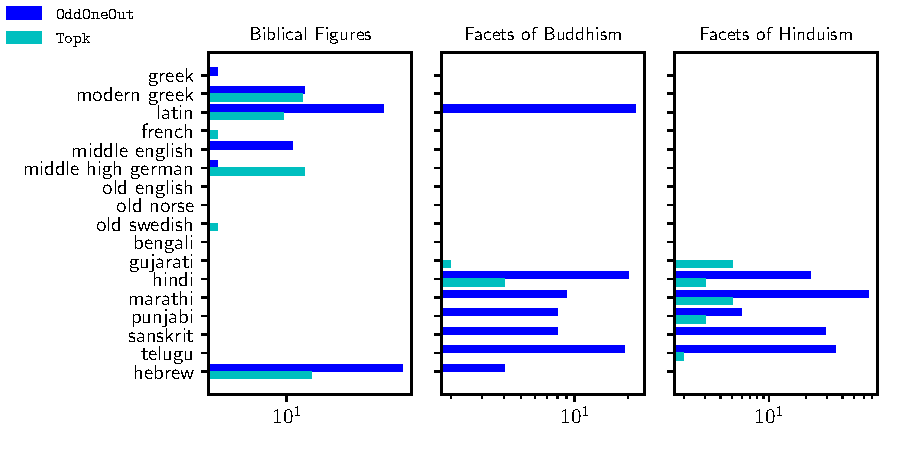
\includegraphics{lct-raw.pdf}}
%\resizebox{6in}{2.75in}{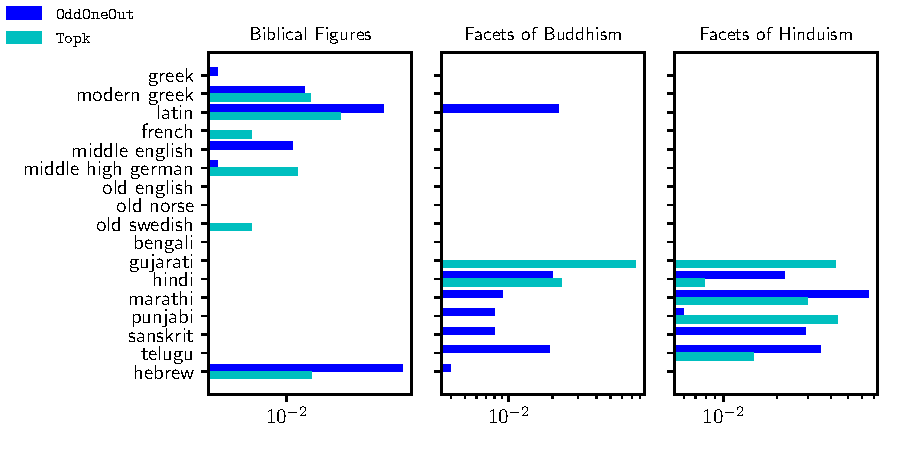
\includegraphics{lct.pdf}}
%
%\caption{
%    (\textbf{Top})
%    High performance on the Biblical Figures category indicates some level of biblical influence via the corpus. 
%    Interestingly, we see that greek embeddings optimized on the Modern Greek test set significantly outperformed the embeddings optimized for the Ancient Greek. 
%    This matches our intuition that things of a biblical nature have had a greater influence on Modern Greek than Ancient Greek.
%    (\textbf{Middle})
%    Though many of the Indic language embeddings performed well on the Facets of Buddhism, 
%    surprisingly so did our Latin and Hebrew embeddings. 
%    This leads us to believe that some Buddhist concepts and words are shared by corpora spanning languages as diverse as Hebrew, Latin, and Hindi. 
%    At the same time, it should also be noted that Latin and Hebrew were two of the largest models trained compared to other classical languages and thus also likely benefit from greater resource richness.
%    (\textbf{Bottom})
%    Similar to Figure \ref{fig:biblical} we see languages more closely related to the topic of the category achieving better performance, in this case primarily the Indic languages. 
%    Interstingly, our Bengali embeddings performed poorly on this category suggesting that the corpus did not refer heavily to the Hindu context.
%}
%\label{fig:downstream}
%\end{figure*}


\section{Conclusion}
\label{sec:discussion}

We introduced the first word vector evaluation methods designed specifically for the low-resource domain, $\OddOneOut$ and $\topk$,
and a method for automatically producing test sets in Wikidata's 581 supported languages.
We believe that Wikidata is an underutilized resource in the NLP evaluation community,
and in particular that it's massively multilingual support can help the NLP community better server under resourced languages.

\ignore{
\fixme{
They also do not use the analogy task to measure performance.
Instead, they use word similarity tasks.
These tasks include datasets based on the English-language WordNet:
WordSim Similarity \citep{zesch2008using}%
%\footnote{
%The WordSim Similarity \citep{zesch2008using} task is the most similar to our proposed $\topk$ and $\OddOneOut$ tasks,
%since they use the wiktionary database\footnote{\url{https://wiktionary.org}} and we use the wikidata database.
%The difference is that: their test set construction technique requires a complicated graph algorithm that requires input from a word bank (they use WordNet for English and GermaNet for German).
%In contrast, our techniques are algorithmically simpler, are easy to interpret, require no external data inputs, and are easily extended to the 400 languages available on wikidata.
%}
WordSim Relatedness \citep{agirre2009study},
and datasets based on human annotation of English language word pairs:
WordSim363 \citep{finkelstein2001placing},
Mechanical Turk \citep{radinsky2011word},
MEN \citep{bruni2012distributional}.
These word similarity tasks are more sensitive to their low-resource experimental design than the analogy task,
but they cannot be easily used in non-English languages because they require the manual generation of new datasets for each language.

Due to Zipf's law, some words will be very infrequent.
Analogies are known to not work well on these infrequently used words.
}

\fixme{
Don't actually make any changes here.
The notes in this section are just for me.
}

\fixme{
    \citet{michel-etal-2020-exploring} study Hiligaynon
}

\fixme{
    There's a simpler way to measure how much each corpus discusses each category:
    simply count the number of times each word from the category is used.
    Can we explain why our method is better than this simpler method?
}
Not yet using wikidata to its fullest extent.
Wikidata categories form a hierarchy.
More accurate evaluations could be done by using all categories in the hierarchy,
weighting top-level categories higher than leaf categories.
This has computational challenges and so we reserve this for future work.

\fixme{Where should this go?
\citet{gonen2020simple} propose a new method for comparing the similarity of two word embeddings in order to find words that are used differently.
Their method assumes that quality word embeddings have already been trained,
and our evaluation metrics provide a way to ensure that this training is done well.
}

\fixme{Where should this go?
\citet{camacho-collados-navigli-2016-find} propose the \texttt{OutlierDetection} metric that is superficially similar to our $\OddOneOut$ metric.
Differences include: their metric is designed to evaluate only a single category relative to itself and is therefore relatively efficient to compute.
Our metric is designed to evaluate many categories relative to all words in the training data.
A naive computation is therefore much more expensive to compute,
and so we introduce a sampling strategy to make the metric computationally feasible.
We also demonstrate that our metric is suitable for the low-resource regime (they only evaluate on datasets with billions of tokens) and make our method available in an easy-to-use open source python library.
}

\fixme{Add this?
Recent work \citet{guntuku2019studying} combines uses the subdivision technique (Section \ref{}) to study how emoji are used differently in different parts of the world.
This technique turns high-resource tasks into low-resource tasks,
and so if you start with a low-resource task it will become even more low-resource.
}

\fixme{
Where does this go?

\citet{al2013polyglot} trained word2vec embeddings on 100 different languages using Wikipedia as the training data.
\citet{grave2018learning} extended this work by training FastText embeddings on 157 languages using data from the Common Crawl project.
\begin{enumerate}
\item
For both papers, the Hindi language had the smallest amount of training data,
with 23 million and 1.8 billion tokens, respectively.
In Section \ref{sec:}, we consider languages with significantly less training data.
For example, the Ancient Hindi language contains only 0.6 million tokens,
and we are still able to generate meaningful word embeddings using our evaluation metrics.

\item
Due to the difficulty of evaluating so many languages, however, the authors evaluate the embeddings only on 10 languages,
and the other 147 remain unevaluated.
\end{enumerate}
}


\fixme{where does this go?
Bias-variance tradeoff in dimensionality of word embeddings \cite{yin2018dimensionality}
}
}


%\section{Related Work}
%\label{sec:related}

%\subsection{Nate}
%
%Look at the way these papers run experiments:
%
%\cite{tifrea2018poincar,meng2019spherical}
%
%Datasets at: \url{https://aclweb.org/aclwiki/Similarity_(State_of_the_art)}
%
%Use wikidata to automatically generate classes: https://www.wikidata.org/wiki/Q43689 
%https://pywikidata.readthedocs.io/en/latest/
%
%wikidata church fathers in latin: \url{https://query.wikidata.org/#SELECT%20%3Fperson%20%3FpersonLabel%0AWHERE%20%7B%0A%20%20%3Fperson%20wdt%3AP361%20wd%3AQ182603.%0A%20%20SERVICE%20wikibase%3Alabel%20%7B%20bd%3AserviceParam%20wikibase%3Alanguage%20%22la%22.%20%7D%0A%7D}
%
%SPARQL Tutorial: \url{https://www.wikidata.org/wiki/Wikidata:SPARQL_tutorial}
%
%Can we use wikidata to automatically generate good evaluations?
%
%\section{Discussion}
%\label{sec:discussion}



%%% End of my stuff 


%\section{Electronically-available resources}
%
%ACL provides this description and accompanying style files at
%\begin{quote}
%\url{https://2020.emnlp.org/files/emnlp2020-templates.zip}
%\end{quote}
%We strongly recommend the use of these style files, which have been appropriately tailored for the EMNLP 2020 proceedings.
%
%\paragraph{\LaTeX-specific details:}
%The templates include the \LaTeX2e{} source (\texttt{\small emnlp2020.tex}),
%the \LaTeX2e{} style file used to format it (\texttt{\small emnlp2020.sty}),
%an ACL bibliography style (\texttt{\small acl\_natbib.bst}),
%an example bibliography (\texttt{\small emnlp2020.bib}),
%and the bibliography for the ACL Anthology (\texttt{\small anthology.bib}).
%
%
%\section{Length of Submission}
%\label{sec:length}
%
%The conference accepts submissions of long papers and short papers.
%Long papers may consist of up to eight (8) pages of content plus unlimited pages for references.
%Upon acceptance, final versions of long papers will be given one additional page -- up to nine (9) pages of content plus unlimited pages for references -- so that reviewers' comments can be taken into account.
%Short papers may consist of up to four (4) pages of content, plus unlimited pages for references.
%Upon acceptance, short papers will be given five (5) pages in the proceedings and unlimited pages for references. 
%For both long and short papers, all illustrations and tables that are part of the main text must be accommodated within these page limits, observing the formatting instructions given in the present document.
%Papers that do not conform to the specified length and formatting requirements are subject to be rejected without review.
%
%The conference encourages the submission of additional material that is relevant to the reviewers but not an integral part of the paper.
%There are two such types of material: appendices, which can be read, and non-readable supplementary materials, often data or code.
%Additional material must be submitted as separate files, and must adhere to the same anonymity guidelines as the main paper.
%The paper must be self-contained: it is optional for reviewers to look at the supplementary material.
%Papers should not refer, for further detail, to documents, code or data resources that are not available to the reviewers.
%Refer to Appendices~\ref{sec:appendix} and \ref{sec:supplemental} for further information. 
%
%Workshop chairs may have different rules for allowed length and whether supplemental material is welcome.
%As always, the respective call for papers is the authoritative source.
%
%
%\section{Anonymity}
%As reviewing will be double-blind, papers submitted for review should not include any author information (such as names or affiliations). Furthermore, self-references that reveal the author's identity, \emph{e.g.},
%\begin{quote}
%We previously showed \citep{Gusfield:97} \ldots
%\end{quote}
%should be avoided. Instead, use citations such as 
%\begin{quote}
%\citet{Gusfield:97} previously showed\ldots
%\end{quote}
%Please do not use anonymous citations and do not include acknowledgements.
%\textbf{Papers that do not conform to these requirements may be rejected without review.}
%
%Any preliminary non-archival versions of submitted papers should be listed in the submission form but not in the review version of the paper.
%Reviewers are generally aware that authors may present preliminary versions of their work in other venues, but will not be provided the list of previous presentations from the submission form.
%
%Once a paper has been accepted to the conference, the camera-ready version of the paper should include the author's names and affiliations, and is allowed to use self-references.
%
%\paragraph{\LaTeX-specific details:}
%For an anonymized submission, ensure that {\small\verb|\aclfinalcopy|} at the top of this document is commented out, and that you have filled in the paper ID number (assigned during the submission process on softconf) where {\small\verb|***|} appears in the {\small\verb|\def\aclpaperid{***}|} definition at the top of this document.
%For a camera-ready submission, ensure that {\small\verb|\aclfinalcopy|} at the top of this document is not commented out.
%
%
%\section{Multiple Submission Policy}
%
%EMNLP 2020 will not consider any paper that is under review in a journal or another conference at the time of submission, and submitted papers must not be submitted elsewhere during the EMNLP 2020 review period. This policy covers all refereed and archival conferences and workshops (e.g., COLING, NeurIPS, ACL workshops). For example, a paper under review at an ACL workshop cannot be dual-submitted to EMNLP 2020. The only exception is that a paper can be dual-submitted to both EMNLP 2020 and an EMNLP workshop which has its submission deadline falling after our original notification date of August 8, 2020. In addition, we will not consider any paper that overlaps significantly in content or results with papers that will be (or have been) published elsewhere. 
%
%Authors submitting more than one paper to EMNLP 2020 must ensure that their submissions do not overlap significantly ($>25$\%) with each other in content or results.
%
%\section{Formatting Instructions}
%
%Manuscripts must be in two-column format.
%Exceptions to the two-column format include the title, authors' names and complete addresses, which must be centered at the top of the first page, and any full-width figures or tables (see the guidelines in Section~\ref{ssec:title-authors}).
%\textbf{Type single-spaced.}
%Start all pages directly under the top margin.
%The manuscript should be printed single-sided and its length should not exceed the maximum page limit described in Section~\ref{sec:length}.
%Pages should be numbered in the version submitted for review, but \textbf{pages should not be numbered in the camera-ready version}.
%
%\paragraph{\LaTeX-specific details:}
%The style files will generate page numbers when {\small\verb|\aclfinalcopy|} is commented out, and remove them otherwise.
%
%
%\subsection{File Format}
%\label{sect:pdf}
%
%For the production of the electronic manuscript you must use Adobe's Portable Document Format (PDF).
%Please make sure that your PDF file includes all the necessary fonts (especially tree diagrams, symbols, and fonts with Asian characters).
%When you print or create the PDF file, there is usually an option in your printer setup to include none, all or just non-standard fonts.
%Please make sure that you select the option of including ALL the fonts.
%\textbf{Before sending it, test your PDF by printing it from a computer different from the one where it was created.}
%Moreover, some word processors may generate very large PDF files, where each page is rendered as an image.
%Such images may reproduce poorly.
%In this case, try alternative ways to obtain the PDF.
%One way on some systems is to install a driver for a postscript printer, send your document to the printer specifying ``Output to a file'', then convert the file to PDF.
%
%It is of utmost importance to specify the \textbf{A4 format} (21 cm x 29.7 cm) when formatting the paper.
%Print-outs of the PDF file on A4 paper should be identical to the hardcopy version.
%If you cannot meet the above requirements about the production of your electronic submission, please contact the publication chairs as soon as possible.
%
%\paragraph{\LaTeX-specific details:}
%PDF files are usually produced from \LaTeX{} using the \texttt{\small pdflatex} command.
%If your version of \LaTeX{} produces Postscript files, \texttt{\small ps2pdf} or \texttt{\small dvipdf} can convert these to PDF.
%To ensure A4 format in \LaTeX, use the command {\small\verb|\special{papersize=210mm,297mm}|}
%in the \LaTeX{} preamble (below the {\small\verb|\usepackage|} commands) and use \texttt{\small dvipdf} and/or \texttt{\small pdflatex}; or specify \texttt{\small -t a4} when working with \texttt{\small dvips}.
%
%\subsection{Layout}
%\label{ssec:layout}
%
%Format manuscripts two columns to a page, in the manner these
%instructions are formatted.
%The exact dimensions for a page on A4 paper are:
%
%\begin{itemize}
%\item Left and right margins: 2.5 cm
%\item Top margin: 2.5 cm
%\item Bottom margin: 2.5 cm
%\item Column width: 7.7 cm
%\item Column height: 24.7 cm
%\item Gap between columns: 0.6 cm
%\end{itemize}
%
%\noindent Papers should not be submitted on any other paper size.
%If you cannot meet the above requirements about the production of your electronic submission, please contact the publication chairs above as soon as possible.
%
%\subsection{Fonts}
%
%For reasons of uniformity, Adobe's \textbf{Times Roman} font should be used.
%If Times Roman is unavailable, you may use Times New Roman or \textbf{Computer Modern Roman}.
%
%Table~\ref{font-table} specifies what font sizes and styles must be used for each type of text in the manuscript.
%
%\begin{table}
%\centering
%\begin{tabular}{lrl}
%\hline \textbf{Type of Text} & \textbf{Font Size} & \textbf{Style} \\ \hline
%paper title & 15 pt & bold \\
%author names & 12 pt & bold \\
%author affiliation & 12 pt & \\
%the word ``Abstract'' & 12 pt & bold \\
%section titles & 12 pt & bold \\
%subsection titles & 11 pt & bold \\
%document text & 11 pt  &\\
%captions & 10 pt & \\
%abstract text & 10 pt & \\
%bibliography & 10 pt & \\
%footnotes & 9 pt & \\
%\hline
%\end{tabular}
%\caption{\label{font-table} Font guide. }
%\end{table}
%
%\paragraph{\LaTeX-specific details:}
%To use Times Roman in \LaTeX2e{}, put the following in the preamble:
%\begin{quote}
%\small
%\begin{verbatim}
%\usepackage{times}
%\usepackage{latexsym}
%\end{verbatim}
%\end{quote}
%
%
%\subsection{Ruler}
%A printed ruler (line numbers in the left and right margins of the article) should be presented in the version submitted for review, so that reviewers may comment on particular lines in the paper without circumlocution.
%The presence or absence of the ruler should not change the appearance of any other content on the page.
%The camera ready copy should not contain a ruler.
%
%\paragraph{Reviewers:}
%note that the ruler measurements may not align well with lines in the paper -- this turns out to be very difficult to do well when the paper contains many figures and equations, and, when done, looks ugly.
%In most cases one would expect that the approximate location will be adequate, although you can also use fractional references (\emph{e.g.}, this line ends at mark $295.5$).
%
%\paragraph{\LaTeX-specific details:}
%The style files will generate the ruler when {\small\verb|\aclfinalcopy|} is commented out, and remove it otherwise.
%
%\subsection{Title and Authors}
%\label{ssec:title-authors}
%
%Center the title, author's name(s) and affiliation(s) across both columns.
%Do not use footnotes for affiliations.
%Place the title centered at the top of the first page, in a 15-point bold font.
%Long titles should be typed on two lines without a blank line intervening.
%Put the title 2.5 cm from the top of the page, followed by a blank line, then the author's names(s), and the affiliation on the following line.
%Do not use only initials for given names (middle initials are allowed).
%Do not format surnames in all capitals (\emph{e.g.}, use ``Mitchell'' not ``MITCHELL'').
%Do not format title and section headings in all capitals except for proper names (such as ``BLEU'') that are
%conventionally in all capitals.
%The affiliation should contain the author's complete address, and if possible, an electronic mail address.
%
%The title, author names and addresses should be completely identical to those entered to the electronical paper submission website in order to maintain the consistency of author information among all publications of the conference.
%If they are different, the publication chairs may resolve the difference without consulting with you; so it is in your own interest to double-check that the information is consistent.
%
%Start the body of the first page 7.5 cm from the top of the page.
%\textbf{Even in the anonymous version of the paper, you should maintain space for names and addresses so that they will fit in the final (accepted) version.}
%
%
%\subsection{Abstract}
%Use two-column format when you begin the abstract.
%Type the abstract at the beginning of the first column.
%The width of the abstract text should be smaller than the
%width of the columns for the text in the body of the paper by 0.6 cm on each side.
%Center the word \textbf{Abstract} in a 12 point bold font above the body of the abstract.
%The abstract should be a concise summary of the general thesis and conclusions of the paper.
%It should be no longer than 200 words.
%The abstract text should be in 10 point font.
%
%\subsection{Text}
%Begin typing the main body of the text immediately after the abstract, observing the two-column format as shown in the present document.
%
%Indent 0.4 cm when starting a new paragraph.
%
%\subsection{Sections}
%
%Format section and subsection headings in the style shown on the present document.
%Use numbered sections (Arabic numerals) to facilitate cross references.
%Number subsections with the section number and the subsection number separated by a dot, in Arabic numerals.
%
%\subsection{Footnotes}
%Put footnotes at the bottom of the page and use 9 point font.
%They may be numbered or referred to by asterisks or other symbols.\footnote{This is how a footnote should appear.}
%Footnotes should be separated from the text by a line.\footnote{Note the line separating the footnotes from the text.}
%
%\subsection{Graphics}
%
%Place figures, tables, and photographs in the paper near where they are first discussed, rather than at the end, if possible.
%Wide illustrations may run across both columns.
%Color is allowed, but adhere to Section~\ref{ssec:accessibility}'s guidelines on accessibility.
%
%\paragraph{Captions:}
%Provide a caption for every illustration; number each one sequentially in the form:
%``Figure 1. Caption of the Figure.''
%``Table 1. Caption of the Table.''
%Type the captions of the figures and tables below the body, using 10 point text.
%Captions should be placed below illustrations.
%Captions that are one line are centered (see Table~\ref{font-table}).
%Captions longer than one line are left-aligned (see Table~\ref{tab:accents}).
%
%\begin{table}
%\centering
%\begin{tabular}{lc}
%\hline
%\textbf{Command} & \textbf{Output}\\
%\hline
%\verb|{\"a}| & {\"a} \\
%\verb|{\^e}| & {\^e} \\
%\verb|{\`i}| & {\`i} \\ 
%\verb|{\.I}| & {\.I} \\ 
%\verb|{\o}| & {\o} \\
%\verb|{\'u}| & {\'u}  \\ 
%\verb|{\aa}| & {\aa}  \\\hline
%\end{tabular}
%\begin{tabular}{lc}
%\hline
%\textbf{Command} & \textbf{Output}\\
%\hline
%\verb|{\c c}| & {\c c} \\ 
%\verb|{\u g}| & {\u g} \\ 
%\verb|{\l}| & {\l} \\ 
%\verb|{\~n}| & {\~n} \\ 
%\verb|{\H o}| & {\H o} \\ 
%\verb|{\v r}| & {\v r} \\ 
%\verb|{\ss}| & {\ss} \\
%\hline
%\end{tabular}
%\caption{Example commands for accented characters, to be used in, \emph{e.g.}, \BibTeX\ names.}\label{tab:accents}
%\end{table}
%
%\paragraph{\LaTeX-specific details:}
%The style files are compatible with the caption and subcaption packages; do not add optional arguments.
%\textbf{Do not override the default caption sizes.}
%
%
%\subsection{Hyperlinks}
%Within-document and external hyperlinks are indicated with Dark Blue text, Color Hex \#000099.
%
%\subsection{Citations}
%Citations within the text appear in parentheses as~\citep{Gusfield:97} or, if the author's name appears in the text itself, as \citet{Gusfield:97}.
%Append lowercase letters to the year in cases of ambiguities.  
%Treat double authors as in~\citep{Aho:72}, but write as in~\citep{Chandra:81} when more than two authors are involved. Collapse multiple citations as in~\citep{Gusfield:97,Aho:72}. 
%
%Refrain from using full citations as sentence constituents.
%Instead of
%\begin{quote}
%  ``\citep{Gusfield:97} showed that ...''
%\end{quote}
%write
%\begin{quote}
%``\citet{Gusfield:97} showed that ...''
%\end{quote}
%
%\begin{table*}
%\centering
%\begin{tabular}{lll}
%\hline
%\textbf{Output} & \textbf{natbib command} & \textbf{Old ACL-style command}\\
%\hline
%\citep{Gusfield:97} & \small\verb|\citep| & \small\verb|\cite| \\
%\citealp{Gusfield:97} & \small\verb|\citealp| & no equivalent \\
%\citet{Gusfield:97} & \small\verb|\citet| & \small\verb|\newcite| \\
%\citeyearpar{Gusfield:97} & \small\verb|\citeyearpar| & \small\verb|\shortcite| \\
%\hline
%\end{tabular}
%\caption{\label{citation-guide}
%Citation commands supported by the style file.
%The style is based on the natbib package and supports all natbib citation commands.
%It also supports commands defined in previous ACL style files for compatibility.
%}
%\end{table*}
%
%\paragraph{\LaTeX-specific details:}
%Table~\ref{citation-guide} shows the syntax supported by the style files.
%We encourage you to use the natbib styles.
%You can use the command {\small\verb|\citet|} (cite in text) to get ``author (year)'' citations as in \citet{Gusfield:97}.
%You can use the command {\small\verb|\citep|} (cite in parentheses) to get ``(author, year)'' citations as in \citep{Gusfield:97}.
%You can use the command {\small\verb|\citealp|} (alternative cite without  parentheses) to get ``author year'' citations (which is useful for  using citations within parentheses, as in \citealp{Gusfield:97}).
%
%
%\subsection{References}
%Gather the full set of references together under the heading \textbf{References}; place the section before any Appendices. 
%Arrange the references alphabetically by first author, rather than by order of occurrence in the text.
%
%Provide as complete a citation as possible, using a consistent format, such as the one for \emph{Computational Linguistics\/} or the one in the  \emph{Publication Manual of the American 
%Psychological Association\/}~\citep{APA:83}.
%Use full names for authors, not just initials.
%
%Submissions should accurately reference prior and related work, including code and data.
%If a piece of prior work appeared in multiple venues, the version that appeared in a refereed, archival venue should be referenced.
%If multiple versions of a piece of prior work exist, the one used by the authors should be referenced.
%Authors should not rely on automated citation indices to provide accurate references for prior and related work.
%
%The following text cites various types of articles so that the references section of the present document will include them.
%\begin{itemize}
%\item Example article in journal: \citep{Ando2005}.
%\item Example article in proceedings, with location: \citep{borschinger-johnson-2011-particle}.
%\item Example article in proceedings, without location: \citep{andrew2007scalable}.
%\item Example arxiv paper: \citep{rasooli-tetrault-2015}. 
%\end{itemize}
%
%
%\paragraph{\LaTeX-specific details:}
%The \LaTeX{} and Bib\TeX{} style files provided roughly follow the American Psychological Association format.
%If your own bib file is named \texttt{\small emnlp2020.bib}, then placing the following before any appendices in your \LaTeX{}  file will generate the references section for you:
%\begin{quote}\small
%\verb|\bibliographystyle{acl_natbib}|\\
%\verb|\bibliography{emnlp2020}|
%\end{quote}
%
%You can obtain the complete ACL Anthology as a Bib\TeX\ file from \url{https://aclweb.org/anthology/anthology.bib.gz}.
%To include both the anthology and your own bib file, use the following instead of the above.
%\begin{quote}\small
%\verb|\bibliographystyle{acl_natbib}|\\
%\verb|\bibliography{anthology,emnlp2020}|
%\end{quote}
%
%
%\subsection{Digital Object Identifiers}
%As part of our work to make ACL materials more widely used and cited outside of our discipline, ACL has registered as a CrossRef member, as a registrant of Digital Object Identifiers (DOIs), the standard for registering permanent URNs for referencing scholarly materials.
%
%All camera-ready references are required to contain the appropriate DOIs (or as a second resort, the hyperlinked ACL Anthology Identifier) to all cited works.
%Appropriate records should be found for most materials in the current ACL Anthology at \url{http://aclanthology.info/}.
%As examples, we cite \citep{goodman-etal-2016-noise} to show you how papers with a DOI will appear in the bibliography.
%We cite \citep{harper-2014-learning} to show how papers without a DOI but with an ACL Anthology Identifier will appear in the bibliography.
%
%\paragraph{\LaTeX-specific details:}
%Please ensure that you use Bib\TeX\ records that contain DOI or URLs for any of the ACL materials that you reference.
%If the Bib\TeX{} file contains DOI fields, the paper title in the references section will appear as a hyperlink to the DOI, using the hyperref \LaTeX{} package.
%
%
%\subsection{Appendices}
%Appendices, if any, directly follow the text and the
%references (but only in the camera-ready; see Appendix~\ref{sec:appendix}).
%Letter them in sequence and provide an informative title:
%\textbf{Appendix A. Title of Appendix}.
%
%\section{Accessibility}
%\label{ssec:accessibility}
%
%In an effort to accommodate people who are color-blind (as well as those printing to paper), grayscale readability is strongly encouraged.
%Color is not forbidden, but authors should ensure that tables and figures do not rely solely on color to convey critical distinctions.
%A simple criterion:
%All curves and points in your figures should be clearly distinguishable without color.
%
%\section{Translation of non-English Terms}
%
%It is also advised to supplement non-English characters and terms with appropriate transliterations and/or translations since not all readers understand all such characters and terms.
%Inline transliteration or translation can be represented in the order of:
%\begin{center}
%\begin{tabular}{c}
%original-form \\
%transliteration \\
%``translation''
%\end{tabular}
%\end{center}
%
%\section{\LaTeX{} Compilation Issues}
%You may encounter the following error during compilation: 
%\begin{quote}
%{\small\verb|\pdfendlink|} ended up in different nesting level than {\small\verb|\pdfstartlink|}.
%\end{quote}
%This happens when \texttt{\small pdflatex} is used and a citation splits across a page boundary.
%To fix this, the style file contains a patch consisting of two lines:
%(1) {\small\verb|\RequirePackage{etoolbox}|} (line 455 in \texttt{\small emnlp2020.sty}), and
%(2) A long line below (line 456 in \texttt{\small emnlp2020.sty}).
%
%If you still encounter compilation issues even with the patch enabled, disable the patch by commenting the two lines, and then disable the \texttt{\small hyperref} package by loading the style file with the \texttt{\small nohyperref} option:
%
%\noindent
%{\small\verb|\usepackage[nohyperref]{emnlp2020}|}
%
%\noindent
%Then recompile, find the problematic citation, and rewrite the sentence containing the citation. (See, {\em e.g.}, \url{http://tug.org/errors.html})
%
%\section*{Acknowledgments}
%
%The acknowledgments should go immediately before the references. Do not number the acknowledgments section.
%Do not include this section when submitting your paper for review.

%\nocite{*}
\bibliographystyle{acl_natbib}
%\interlinepenalty=10000
\bibliography{emnlp2020}


\end{document}
